\documentclass[UTF8]{ctexart}
\usepackage{datetime}
\usepackage{geometry}
\usepackage{array}
\usepackage{graphicx}
% 封面
\geometry{a4paper,left=1cm,right=2cm,top=1cm,bottom=1cm}
\title{\Huge 电工电子实验中心}
\author{\Large 实验报告}
\begin{document}
\maketitle
\vspace{6\baselineskip}
\renewcommand\arraystretch{1.5}
\begin{table}[h]
    \centering
    \Large
    \setlength{\tabcolsep}{5mm}{
        \begin{tabular}{rcrc}
            课程名称: & 数字电子技术 & 实验项目: & 同步时序电路 \\

            姓名:     & xxx       & 学号:     & xxxxxxxxx    \\

            班级:     & xxxxxxx      & 日期:     & \today       \\

            地点:     & 3313         & 成绩:     &              \\
        \end{tabular}}
\end{table}

\vspace{10\baselineskip}

\centering
南京航空航天大学 \\
\newpage


% 内容页
\begin{enumerate}
    \large
    \vspace{1\baselineskip}
    \item 原理及设计方案:  \\
          \begin{itemize}
              \item [1.] 设计步骤 \\
                    \begin{center}
                        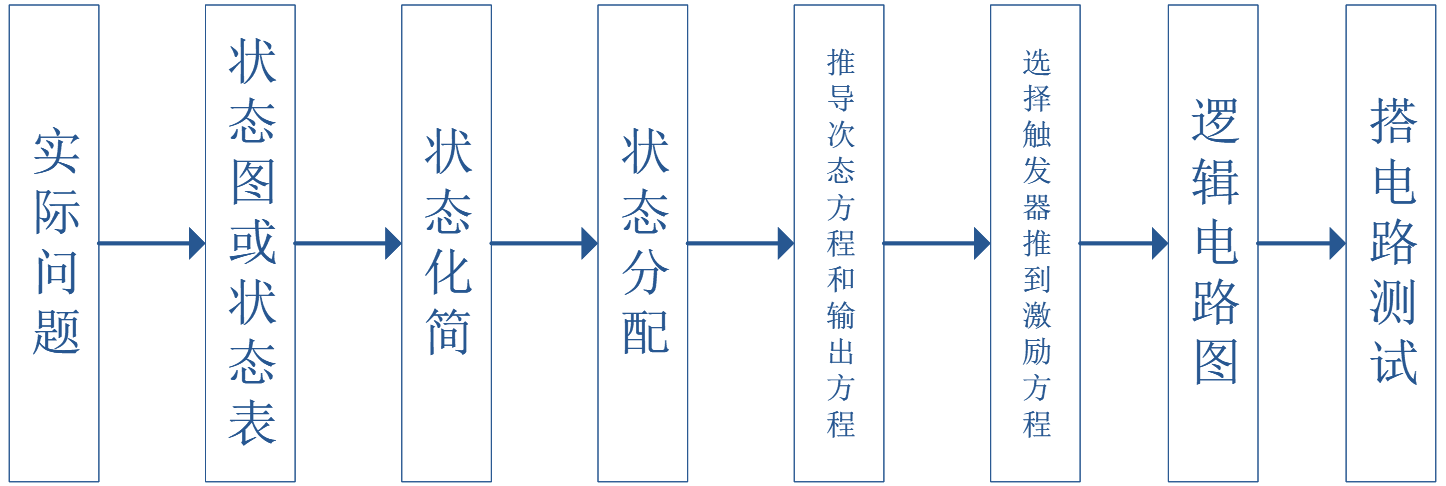
\includegraphics[scale=0.6]{1.png}
                        \label{fig:label}
                    \end{center}

              \item [2.] 状态图 \\
                    \begin{center}
                        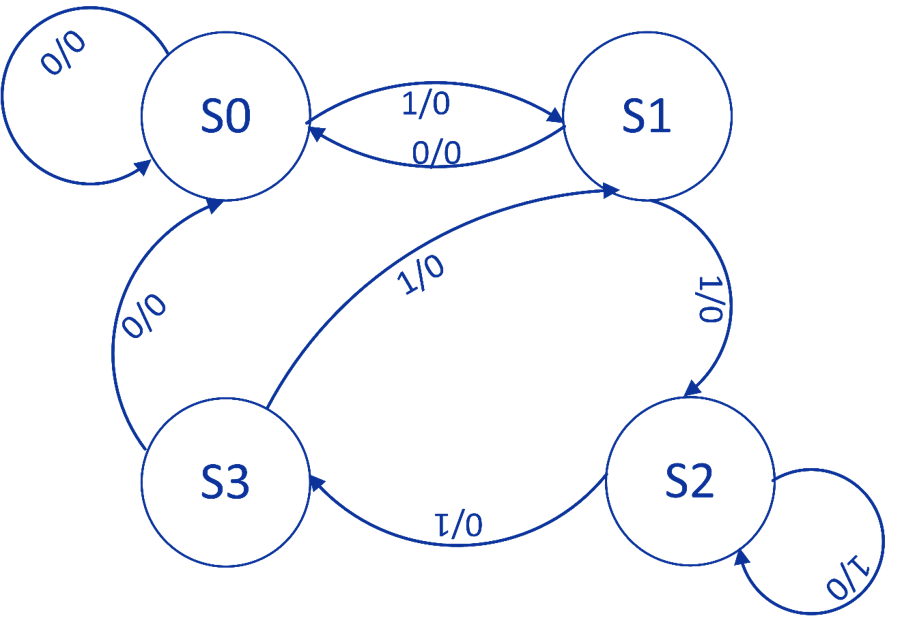
\includegraphics[scale = 0.6]{2.png}
                        \label{fig:label}
                    \end{center}

              \item [3.] 状态表              \\
                    \begin{center}
                        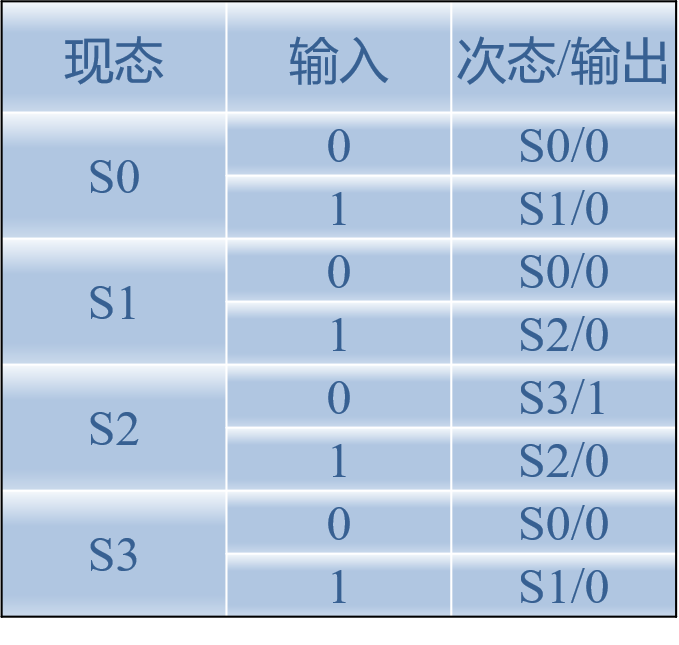
\includegraphics[scale = 0.6]{3.png}
                        \label{fig:label}
                    \end{center}
              \item [4.] 化简后状态表              \\
                    \begin{center}
                        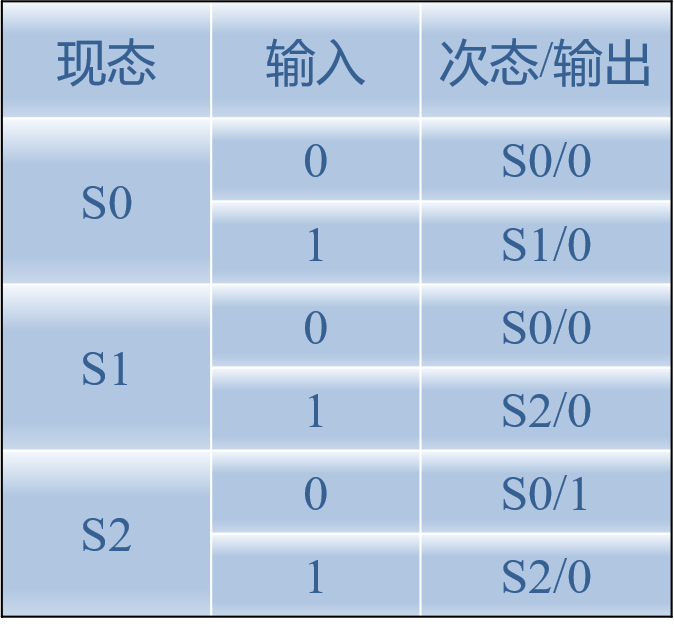
\includegraphics[scale = 0.6]{4.png}
                        \label{fig:label}
                    \end{center}
              \item [5.] 编码状态表              \\
                    \begin{center}
                        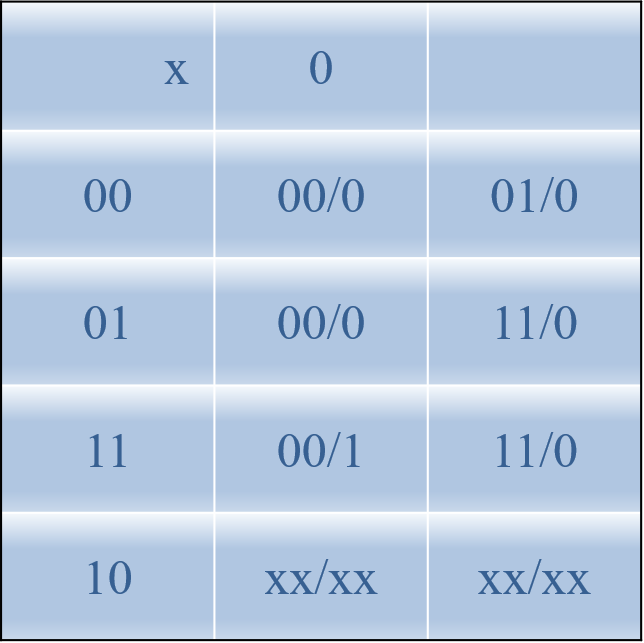
\includegraphics[scale = 0.6]{5.png}
                        \label{fig:label}
                    \end{center}
              \item [6.] 次态卡诺图和输出卡诺图            \\
                    \begin{center}
                        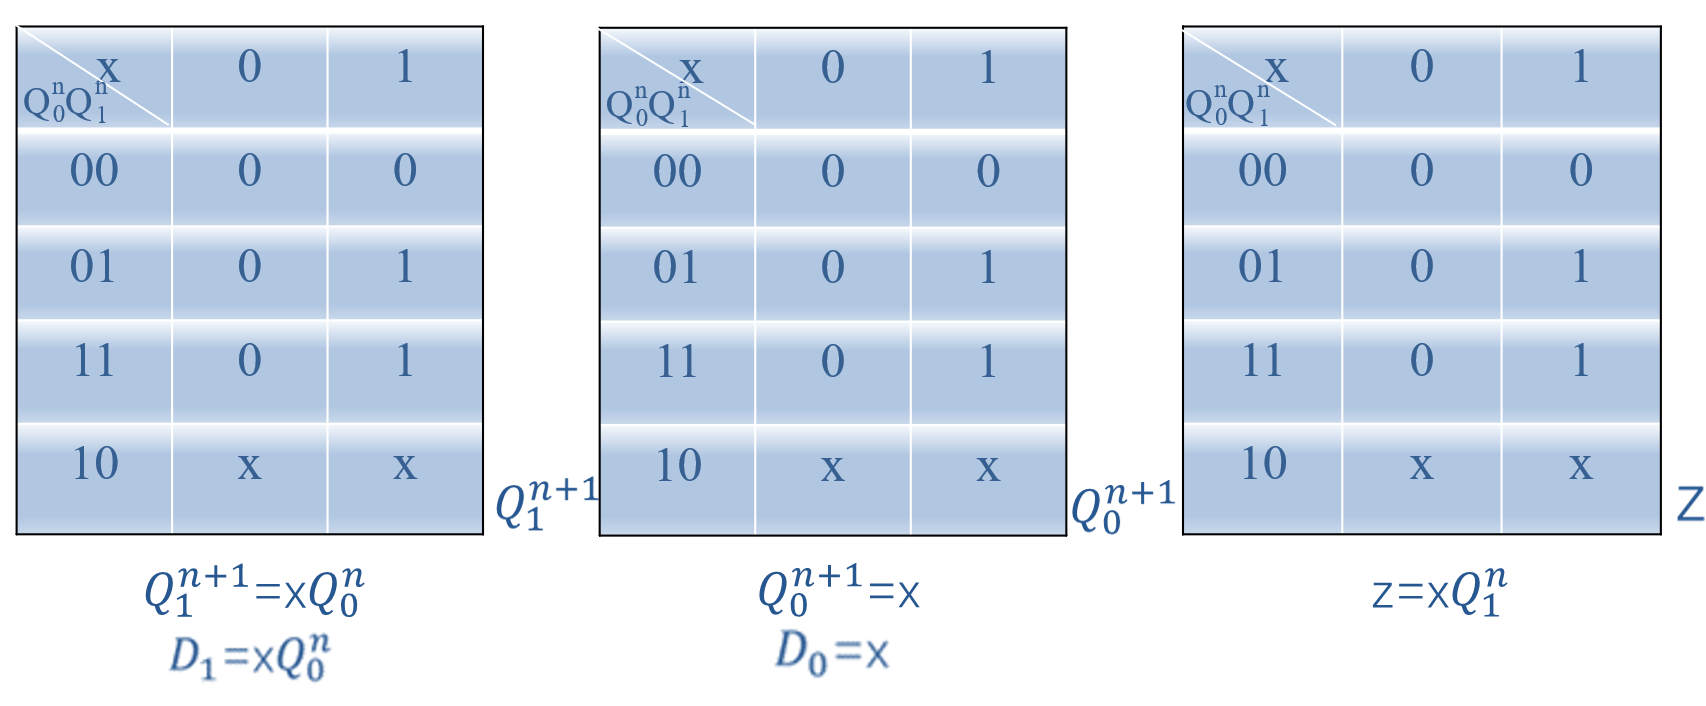
\includegraphics[scale = 0.6]{6.png}
                        \label{fig:label}
                    \end{center}
              \item [7.] 选择D触发器作为状态寄存器获得激励方程
                    \begin{center}
                        $D_1 = xQ_0^n$\\
                        $D_0 = x$\\
                    \end{center}
                    \newpage
              \item [8.] 画出逻辑电路图
                    \begin{center}
                        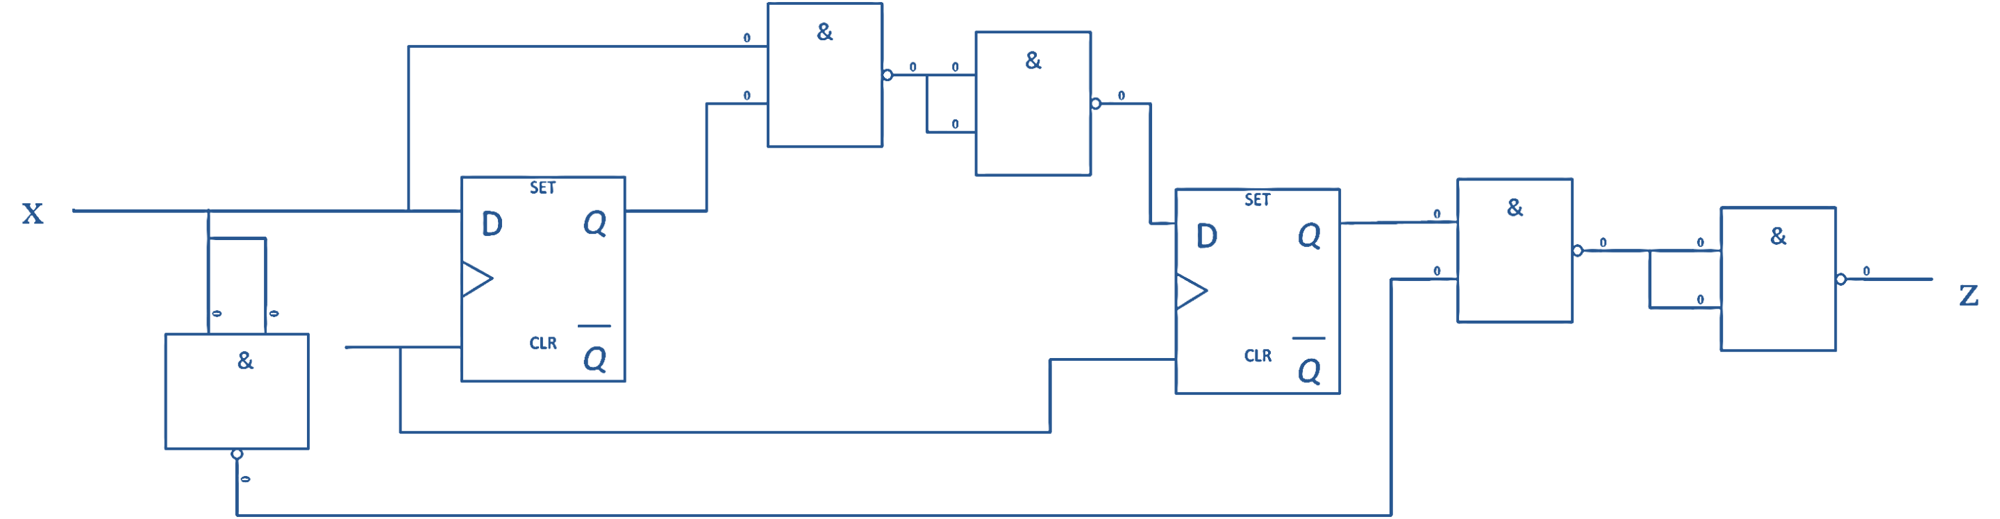
\includegraphics[scale = 0.4]{7.png}
                        \label{fig:label}
                    \end{center}
          \end{itemize}
    \item 计算及仿真:  \\
          \begin{center}
              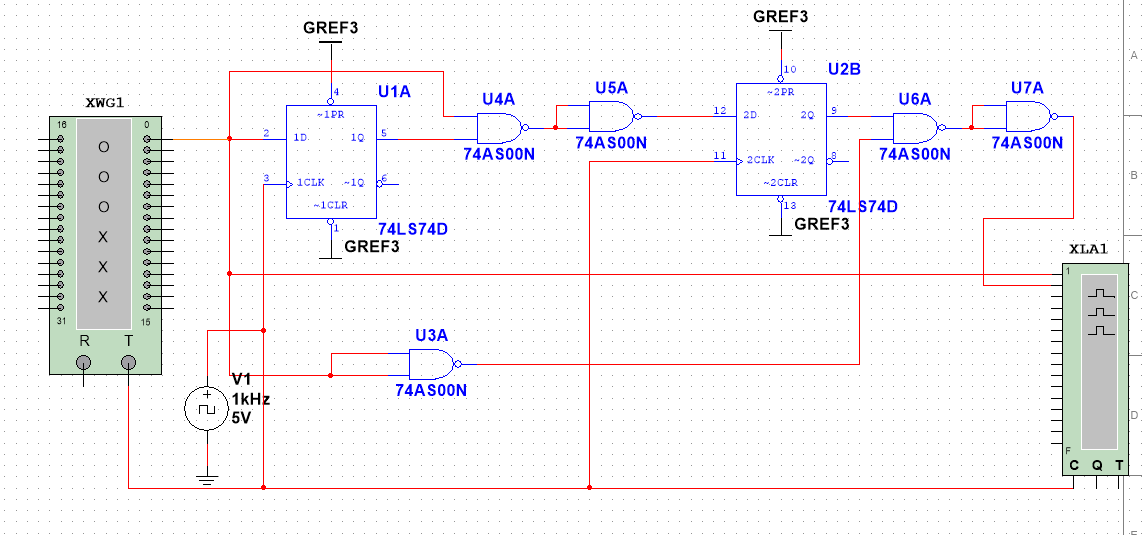
\includegraphics[scale = 0.4]{10.png}
              \label{fig:label}
          \end{center}
          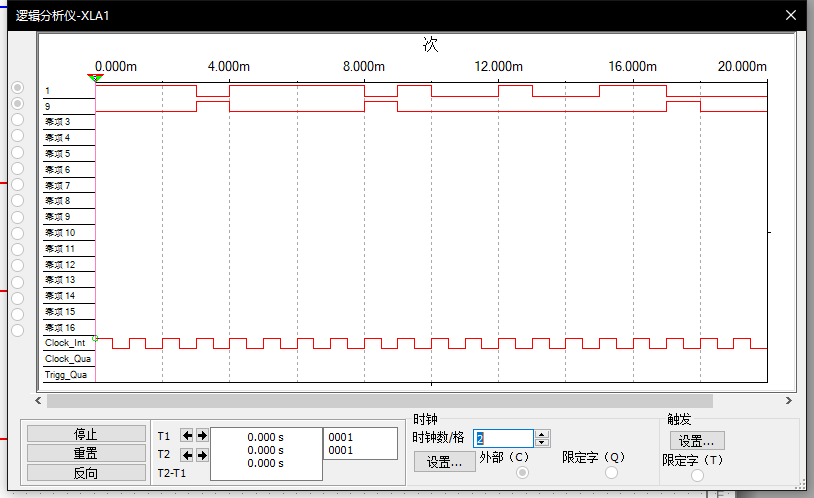
\includegraphics[scale = 0.3]{8.png}
          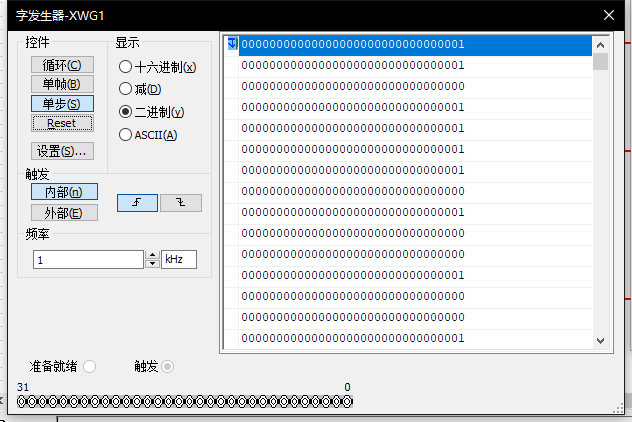
\includegraphics[scale = 0.4]{9.png}



    \item  实验目的: \\

          \begin{itemize}
              \item [1.]  加深理解触发器的特征。
              \item [2.]  掌握同步时序电路的设计与调试方法。
          \end{itemize}
          \newpage
    \item  实验过程及数据分析:  \\

\end{enumerate}
\end{document}